\begin{problem}[问题1.1]
1687年牛顿首先发表了他的剪切流动的实验结果,他的实验是在两相距$h$的平行板之间充满粘性流体后进行的,如图\ref{experiment}. 令下平行板固定不动,而使上平板在其自身平面以等速$U$向右运动. 实验指出, 平衡后作用于平板上的力与速度$U$
及平板面积$A$成正比,与平板间距$h$成反比,即
\[
F = \mu \frac{U}{h}A {~}\textrm{或}{~} \tau = \frac{F}{A}=\mu\frac{U}{h}
\]
讨论在牛顿剪切流动的实验中, 作用于上平板的外力在流体运动平衡前随时间的变化.
\end{problem}


\begin{solution}
\begin{figure}[!htb]
\begin{minipage}[c]{.5\textwidth}
\centering
%\includegraphics[width=0.9\textwidth]{experiment.pdf}
\usetikzlibrary{%
    decorations.pathreplacing,%
    decorations.pathmorphing,arrows
}

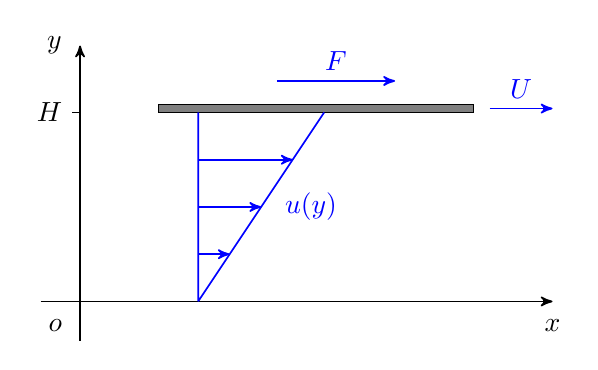
\begin{tikzpicture}
\draw[->,semithick, >=stealth'] (-0.5,0)--(6,0) node[below=3pt]{$x$};
\draw[->,semithick, >=stealth'] (0,-0.5)--(0,3.25)node[left=3pt]{$y$};
\draw[semithick] (-0.1,2.4)node[left]{$H$}--(0,2.4);
\node[below left=3pt] at (0,0){$o$};

\draw[fill=gray] (1,2.4) rectangle (5,2.5);
\draw[->,semithick, >=stealth',blue] (5.2,2.45)--(6,2.45)node[midway,above]{$U$};
\draw[->,semithick, >=stealth',blue] (2.5,2.8)--(4,2.8)node[midway,above]{$F$};

\draw[semithick,blue] (1.5,0)--(1.5,2.4) (1.5,0)--(3.1,2.4);

\draw[->,semithick, >=stealth',blue](1.5,0.6)--(1.9,0.6);
\draw[->,semithick, >=stealth',blue](1.5,1.2)--(2.3,1.2) node[right=5pt]{$u(y)$};
\draw[->,semithick, >=stealth',blue](1.5,1.8)--(2.7,1.8);

\end{tikzpicture}
\caption{\label{experiment}剪切流实验}
\end{minipage}%
\begin{minipage}[c]{.5\textwidth}
\centering
\usetikzlibrary{%
    decorations.pathreplacing,%
    decorations.pathmorphing,arrows
}

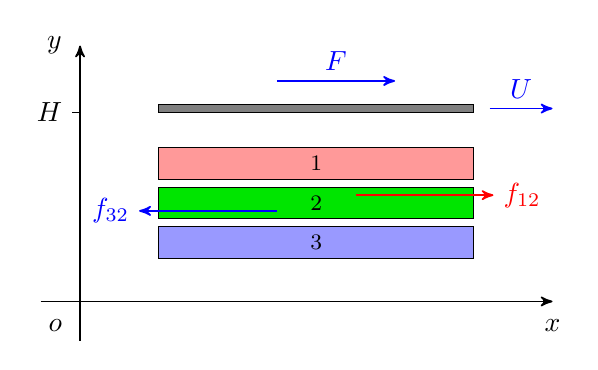
\begin{tikzpicture}
\draw[->,semithick, >=stealth'] (-0.5,0)--(6,0) node[below=3pt]{$x$};
\draw[->,semithick, >=stealth'] (0,-0.5)--(0,3.25)node[left=3pt]{$y$};
\draw[semithick] (-0.1,2.4)node[left]{$H$}--(0,2.4);
\node[below left=3pt] at (0,0){$o$};

\draw[fill=gray] (1,2.4) rectangle (5,2.5);
\draw[->,semithick, >=stealth',blue] (5.2,2.45)--(6,2.45)node[midway,above]{$U$};
\draw[->,semithick, >=stealth',blue] (2.5,2.8)--(4,2.8)node[midway,above]{$F$};

\draw[fill=red!40] (1,1.55) rectangle (5,1.95) node[midway,font=\footnotesize]{1};
\draw[fill=green!90!black] (1,1.05) rectangle (5,1.45)  node[midway,font=\footnotesize]{2};
\draw[fill=blue!40] (1,0.55) rectangle (5,0.95)  node[midway,font=\footnotesize]{3};

\draw[->,semithick, >=stealth',blue] (2.5,1.15)--(0.75,1.15) node[left]{$f_{32}$};
\draw[->,semithick, >=stealth',red] (3.5,1.35)--(5.25,1.35) node[right]{$f_{12}$};


\end{tikzpicture}
%\includegraphics[width=0.9\textwidth]{layers.pdf}
\caption{\label{layers}微元受力分析}
\end{minipage}
\end{figure}

\textbf{解:}如图\ref{layers}所示, 取高度为$\Delta h$面积为$A$的三个微元层, 标记为1,2,3. 设1,2,3层的速度分别为$v_1$,$v_2$,$v_3$; 微元1对微元2的作用力为$f_{12}$, 微元3对微元2的作用力为$f_{32}$. 则有
\begin{equation}
f_{12} = \mu \frac{v1-v2}{\Delta h}A=\mu \frac{du(y_{12})}{dy}A, {~}f_{32} = \mu \frac{v_3-v_2}{\Delta h}A= \mu \frac{du(y_{32})}{dy}A
\end{equation}
则对于微元2有
\begin{equation}
\frac{du(y_2)}{dt} = \frac{f_{12} - f_{32}}{\rho A \Delta h}
= \frac{f_{12} - f_{23}}{\rho A \Delta h} = \frac{\mu}{\rho}\frac{d^2u(y_2)}{dy^2}
\end{equation}
因此有以下微分方程组
\begin{equation}\label{diff}
\begin{dcases}
\frac{\partial u(y,t)}{\partial t} = \frac{\mu}{\rho} \frac{\partial ^2 u(y,t)}{\partial y^2} \\
\frac{\partial u(y,t)}{\partial x} = 0 \\
u(0,t) = 0, {~}u(H,t) = U, {~}u(y<H)|_{t=0} = 0
\end{dcases}
\end{equation}

\noindent\textbf{数值模拟法求解}

根据以上分析, 将微分方程组式(\ref{diff})离散成差分格式,并通过编程计算,可得到外力F随时间的近似变化. 例如, 以273.15K下的水为例, 并令$H=0.05$m, $U=1$m/s.将高$H=0.05$m的水等高的划分成$n = 100$层. 以$dt = 0.02$为时间步长, 每个时间步内,通过计算各层间的黏性力,来得到各层的加速度, 从而更新各层的速度. 图\ref{force}是外力$F$随时间的变化, 其平衡值为0.0354, 与理论值$F=\mu U/H = 1750\times 10^{-6}\times 1/0.05 = 0.0350$相差1.14\%. 图\ref{velocity}为不同时刻速度沿y方向的分布,$t=1000$s时速度成线性分布,这与牛顿所给出的结果是一致的.该计算所使用的程序见附录\ref{sec:ShearExperiment}.

\begin{figure}[!htb]
\begin{minipage}[c]{.5\textwidth}
\centering
%\includegraphics[width=0.9\textwidth]{force.pdf}
\begin{tikzpicture}
\begin{axis}[width=0.9\textwidth,height=0.75\textwidth,
xmin=-2,
xmax=1000,
xlabel={Time(s)},
ymin=-0.002,
ymax=0.5,
ytick={0.0354,0.1,0.2,0.3,0.4,0.5},
yticklabels={0.035,0.1,0.2,0.3,0.4,0.5},
ylabel={Force(N)},
yticklabel style={font=\scriptsize},
xticklabel style={font=\scriptsize},
xlabel style={font=\footnotesize},
ylabel style={font=\footnotesize}
]

\addplot[color=blue,dashed,domain=0:1000]{0.0354};
\addplot[no markers, smooth,red]
  table[row sep=crcr]{%
0	3.5\\
1	0.734305374682564\\
2	0.523454217532651\\
3	0.428561127577308\\
4	0.371650449039231\\
5	0.332686255938993\\
6	0.303865383638172\\
7	0.281434416211684\\
8	0.263334834391634\\
9	0.248330990656227\\
10	0.235630383921036\\
11	0.22469825068544\\
12	0.215158928170908\\
13	0.206739748990519\\
14	0.199237365019313\\
15	0.192496619886634\\
16	0.18639679376219\\
17	0.180842361161256\\
18	0.175756610150057\\
19	0.171077131664224\\
20	0.166752563890995\\
30	0.136190153414217\\
40	0.117960271744588\\
50	0.105515537739813\\
60	0.0963273400535577\\
70	0.0891852753705457\\
80	0.0834276368124073\\
90	0.0786581485082112\\
100	0.0746231321090408\\
110	0.071151732712454\\
120	0.0681242116812327\\
130	0.0654539500916878\\
140	0.063076652996078\\
150	0.0609435643755754\\
160	0.0590170301023314\\
170	0.0572674971715746\\
180	0.05567142669425\\
190	0.0542098088997883\\
200	0.0528670869882919\\
210	0.0516303658438363\\
220	0.050488823410101\\
230	0.0494332686621414\\
240	0.0484558070013036\\
250	0.0475495851612274\\
260	0.0467085954262233\\
270	0.0459275243693893\\
280	0.0452016351782601\\
290	0.0445266754331262\\
300	0.0438988042531376\\
310	0.0433145342402184\\
320	0.0427706847774666\\
330	0.0422643440804263\\
340	0.0417928380306875\\
350	0.041353704295644\\
360	0.0409446705955765\\
370	0.0405636362488099\\
380	0.040208656329467\\
390	0.0398779279264925\\
400	0.0395697781094865\\
410	0.0392826532955367\\
420	0.0390151097787045\\
430	0.0387658052351657\\
440	0.0385334910562569\\
450	0.0383170053917145\\
460	0.0381152668084958\\
470	0.0379272684883656\\
480	0.0377520729012517\\
490	0.0375888069021253\\
500	0.0374366572075955\\
510	0.0372948662150735\\
520	0.0371627281326662\\
530	0.0370395853922217\\
540	0.0369248253213969\\
550	0.0368178770534715\\
560	0.0367182086559546\\
570	0.0366253244610162\\
580	0.0365387625824411\\
590	0.0364580926052134\\
600	0.036382913435103\\
610	0.0363128512966771\\
620	0.0362475578691363\\
630	0.0361867085502058\\
640	0.036130000839075\\
650	0.0360771528300723\\
660	0.0360279018093647\\
670	0.035982002947553\\
680	0.0359392280815364\\
690	0.0358993645795062\\
700	0.03586221428335\\
710	0.0358275925231648\\
720	0.0357953271989354\\
730	0.0357652579247886\\
740	0.0357372352315385\\
750	0.0357111198235532\\
760	0.0356867818862336\\
770	0.0356641004406372\\
780	0.0356429627420598\\
790	0.0356232637195538\\
800	0.0356049054536047\\
810	0.035587796689372\\
820	0.0355718523830569\\
830	0.0355569932791549\\
840	0.0355431455164816\\
850	0.0355302402610206\\
860	0.035518213363754\\
870	0.0355070050417907\\
880	0.0354965595811954\\
890	0.0354868250600427\\
900	0.0354777530903255\\
910	0.0354692985774287\\
920	0.03546141949597\\
930	0.0354540766809042\\
940	0.0354472336328409\\
950	0.0354408563366115\\
960	0.0354349130921934\\
970	0.0354293743571326\\
980	0.0354242125996927\\
990	0.0354194021620075\\
1000	0.0354149191325349\\
};
\end{axis}
\end{tikzpicture}%

\caption{\label{force}外力$F$随时间的变化}
\end{minipage}%
\begin{minipage}[c]{.5\textwidth}
\centering
%\includegraphics[width=0.85\textwidth]{velocity.pdf}
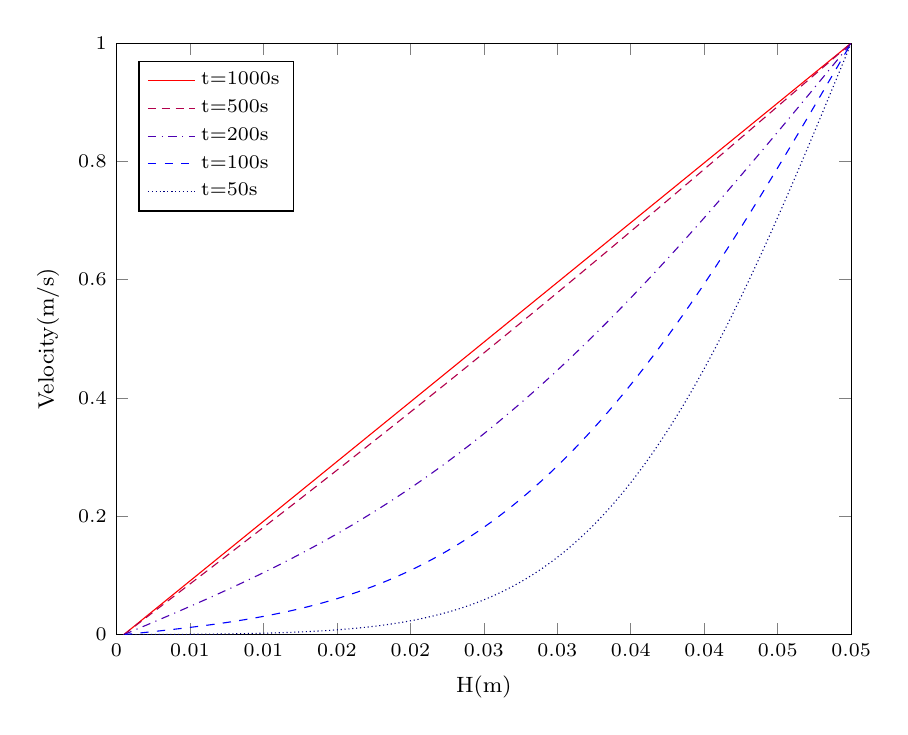
\begin{tikzpicture}
\begin{axis}[width=0.9\textwidth,height=0.75\textwidth,
xmin=0,
xmax=0.05,
xlabel={H(m)},
ymin=0,
ymax=1,
ylabel={Velocity(m/s)},
yticklabel style={font=\scriptsize},
xticklabel style={font=\scriptsize},
xlabel style={font=\footnotesize},
ylabel style={font=\footnotesize},
      scaled x ticks = false,
      xticklabel style={/pgf/number format/fixed,
      /pgf/number format/1000 sep = \thinspace},
anchor=left of south west,
legend style={legend pos=north west,font=\scriptsize,legend cell align=left},
]

\addplot [color=red,solid]
  table[row sep=crcr]{%
0.0005	0\\
0.001	0.0100834743507922\\
0.0015	0.0201669663585983\\
0.002	0.0302504936626533\\
0.0025	0.0403340738666517\\
0.003	0.0504177245210224\\
0.0035	0.0605014631052565\\
0.004	0.0705853070103073\\
0.0045	0.0806692735210791\\
0.005	0.0907533797990224\\
0.0055	0.100837642864854\\
0.006	0.110922079581419\\
0.0065	0.121006706636711\\
0.007	0.131091540527067\\
0.0075	0.141176597540562\\
0.008	0.1512618937406\\
0.0085	0.16134744494975\\
0.009	0.171433266733804\\
0.0095	0.18151937438611\\
0.01	0.191605782912171\\
0.0105	0.201692507014535\\
0.011	0.211779561077991\\
0.0115	0.221866959155087\\
0.012	0.231954714951977\\
0.0125	0.242042841814621\\
0.013	0.252131352715349\\
0.0135	0.262220260239795\\
0.014	0.272309576574229\\
0.0145	0.282399313493281\\
0.015	0.292489482348091\\
0.0155	0.302580094054875\\
0.016	0.312671159083934\\
0.0165	0.322762687449112\\
0.017	0.332854688697714\\
0.0175	0.342947171900891\\
0.018	0.353040145644506\\
0.0185	0.36313361802049\\
0.019	0.373227596618692\\
0.0195	0.383322088519241\\
0.02	0.393417100285411\\
0.0205	0.403512637957018\\
0.021	0.413608707044333\\
0.0215	0.423705312522539\\
0.022	0.433802458826718\\
0.0225	0.443900149847385\\
0.023	0.453998388926574\\
0.0235	0.464097178854467\\
0.024	0.474196521866593\\
0.0245	0.484296419641567\\
0.025	0.494396873299407\\
0.0255	0.504497883400406\\
0.026	0.514599449944563\\
0.0265	0.524701572371586\\
0.027	0.534804249561458\\
0.0275	0.544907479835562\\
0.028	0.555011260958372\\
0.0285	0.565115590139704\\
0.029	0.575220464037524\\
0.0295	0.585325878761319\\
0.03	0.595431829876004\\
0.0305	0.605538312406399\\
0.031	0.615645320842232\\
0.0315	0.625752849143687\\
0.032	0.635860890747489\\
0.0325	0.645969438573511\\
0.033	0.656078485031903\\
0.0335	0.666188022030734\\
0.034	0.676298040984141\\
0.0345	0.686408532820973\\
0.035	0.696519487993927\\
0.0355	0.706630896489156\\
0.036	0.716742747836361\\
0.0365	0.726855031119325\\
0.037	0.736967734986909\\
0.0375	0.747080847664482\\
0.038	0.757194356965775\\
0.0385	0.767308250305153\\
0.039	0.777422514710286\\
0.0395	0.787537136835215\\
0.04	0.797652102973785\\
0.0405	0.807767399073449\\
0.041	0.817883010749417\\
0.0415	0.827998923299141\\
0.042	0.838115121717119\\
0.0425	0.848231590710003\\
0.043	0.858348314711998\\
0.0435	0.868465277900539\\
0.044	0.878582464212219\\
0.0445	0.888699857358965\\
0.045	0.898817440844438\\
0.0455	0.908935197980645\\
0.046	0.919053111904742\\
0.0465	0.929171165596011\\
0.047	0.939289341893001\\
0.0475	0.949407623510809\\
0.048	0.95952599305848\\
0.0485	0.969644433056524\\
0.049	0.979762925954512\\
0.0495	0.989881454148749\\
0.05	1\\
};
\addlegendentry{t=1000s};

\addplot [color=red!70!blue,densely dashed]
  table[row sep=crcr]{%
0.0005	0\\
0.001	0.00950594677208322\\
0.0015	0.0190124926765428\\
0.002	0.0285202362426647\\
0.0025	0.0380297747941604\\
0.003	0.0475417038478953\\
0.0035	0.0570566165144347\\
0.004	0.0665751029010088\\
0.0045	0.0760977495174991\\
0.005	0.0856251386860422\\
0.0055	0.0951578479548454\\
0.006	0.104696449516803\\
0.0065	0.1142415096335\\
0.007	0.123793588065179\\
0.0075	0.133353237507248\\
0.008	0.142921003033892\\
0.0085	0.152497421549352\\
0.009	0.162083021247419\\
0.0095	0.171678321079691\\
0.01	0.181283830233124\\
0.0105	0.190900047617406\\
0.011	0.200527461362672\\
0.0115	0.210166548328056\\
0.012	0.219817773621581\\
0.0125	0.229481590131881\\
0.013	0.239158438072197\\
0.0135	0.248848744537142\\
0.014	0.25855292307265\\
0.0145	0.268271373259566\\
0.015	0.27800448031128\\
0.0155	0.287752614685815\\
0.016	0.297516131712769\\
0.0165	0.307295371235467\\
0.017	0.317090657268707\\
0.0175	0.326902297672422\\
0.018	0.336730583841611\\
0.0185	0.346575790412824\\
0.019	0.356438174987524\\
0.0195	0.366317977872585\\
0.02	0.376215421838197\\
0.0205	0.386130711893424\\
0.021	0.396064035079634\\
0.0215	0.406015560282015\\
0.022	0.415985438059367\\
0.0225	0.425973800492337\\
0.023	0.435980761050262\\
0.0235	0.446006414476744\\
0.024	0.456050836694068\\
0.0245	0.466114084726585\\
0.025	0.476196196643103\\
0.0255	0.486297191518378\\
0.026	0.496417069413718\\
0.0265	0.506555811376739\\
0.027	0.516713379460263\\
0.0275	0.52688971676034\\
0.028	0.537084747473372\\
0.0285	0.547298376972254\\
0.029	0.557530491901482\\
0.0295	0.567780960291122\\
0.03	0.578049631689525\\
0.0305	0.588336337314655\\
0.031	0.598640890223883\\
0.0315	0.608963085502077\\
0.032	0.619302700467788\\
0.0325	0.62965949489734\\
0.033	0.640033211266585\\
0.0335	0.650423575010099\\
0.034	0.660830294797531\\
0.0345	0.671253062826855\\
0.035	0.681691555134212\\
0.0355	0.692145431920034\\
0.036	0.702614337891134\\
0.0365	0.713097902618396\\
0.037	0.723595740909722\\
0.0375	0.734107453197858\\
0.038	0.744632625942704\\
0.0385	0.755170832047702\\
0.039	0.765721631289893\\
0.0395	0.776284570763194\\
0.04	0.786859185334467\\
0.0405	0.797444998111905\\
0.041	0.80804152092527\\
0.0415	0.8186482548175\\
0.042	0.829264690547188\\
0.0425	0.839890309101429\\
0.043	0.85052458221851\\
0.0435	0.861166972919934\\
0.044	0.871816936051217\\
0.0445	0.882473918830939\\
0.045	0.893137361407474\\
0.0455	0.903806697422854\\
0.046	0.914481354583187\\
0.0465	0.925160755235063\\
0.047	0.935844316947359\\
0.0475	0.946531453097862\\
0.048	0.957221573464119\\
0.0485	0.967914084817915\\
0.049	0.978608391522779\\
0.0495	0.989303896133924\\
0.05	1\\
};
\addlegendentry{t=500s};

\addplot [color=red!30!blue,dashdotted]
  table[row sep=crcr]{%
0.0005	0\\
0.001	0.00524135730404738\\
0.0015	0.0104873917269853\\
0.002	0.0157427765460405\\
0.0025	0.0210121773555081\\
0.003	0.0263002482262919\\
0.0035	0.0316116278666871\\
0.004	0.0369509357848836\\
0.0045	0.0423227684537193\\
0.005	0.0477316954782777\\
0.0055	0.053182255767003\\
0.006	0.0586789537070958\\
0.0065	0.0642262553450529\\
0.007	0.069828584573328\\
0.0075	0.0754903193242138\\
0.008	0.081215787772176\\
0.0085	0.0870092645460141\\
0.009	0.0928749669523733\\
0.0095	0.0988170512122895\\
0.01	0.104839608712614\\
0.0105	0.110946662274333\\
0.011	0.117142162439984\\
0.0115	0.123429983782523\\
0.012	0.129813921238225\\
0.0125	0.136297686466328\\
0.013	0.142884904238376\\
0.0135	0.149579108860355\\
0.014	0.156383740630925\\
0.0145	0.163302142339239\\
0.015	0.170337555805998\\
0.0155	0.177493118471588\\
0.016	0.184771860035317\\
0.0165	0.192176699149903\\
0.017	0.199710440175581\\
0.0175	0.207375769998274\\
0.018	0.215175254916483\\
0.0185	0.223111337601625\\
0.019	0.231186334136712\\
0.0195	0.239402431138336\\
0.02	0.247761682967034\\
0.0205	0.2562660090312\\
0.021	0.264917191189754\\
0.0215	0.27371687125884\\
0.022	0.282666548627867\\
0.0225	0.291767577990214\\
0.023	0.301021167193924\\
0.0235	0.310428375217702\\
0.024	0.319990110277503\\
0.0245	0.32970712806892\\
0.025	0.339580030150544\\
0.0255	0.349609262473348\\
0.026	0.359795114061072\\
0.0265	0.370137715846427\\
0.027	0.380637039667807\\
0.0275	0.391292897431034\\
0.028	0.40210494044047\\
0.0285	0.413072658903641\\
0.029	0.42419538161327\\
0.0295	0.435472275810418\\
0.03	0.446902347232143\\
0.0305	0.458484440346829\\
0.031	0.470217238780055\\
0.0315	0.482099265933547\\
0.032	0.494128885799475\\
0.0325	0.506304303971984\\
0.033	0.518623568857529\\
0.0335	0.531084573085222\\
0.034	0.543685055118016\\
0.0345	0.556422601065199\\
0.035	0.569294646696252\\
0.0355	0.582298479655749\\
0.036	0.595431241878577\\
0.0365	0.608689932204324\\
0.037	0.622071409189295\\
0.0375	0.635572394114195\\
0.038	0.649189474185076\\
0.0385	0.662919105924777\\
0.039	0.676757618751609\\
0.0395	0.690701218741684\\
0.04	0.704745992570825\\
0.0405	0.718887911631618\\
0.041	0.733122836320764\\
0.0415	0.747446520491481\\
0.042	0.761854616065348\\
0.0425	0.776342677797589\\
0.043	0.790906168189445\\
0.0435	0.805540462540926\\
0.044	0.820240854136916\\
0.0445	0.835002559559259\\
0.045	0.849820724117176\\
0.0455	0.864690427388051\\
0.046	0.879606688860389\\
0.0465	0.894564473670457\\
0.047	0.909558698423927\\
0.0475	0.924584237093608\\
0.048	0.939635926984183\\
0.0485	0.954708574754672\\
0.049	0.969796962489245\\
0.0495	0.984895853806844\\
0.05	1\\
};
\addlegendentry{t=200s};





\addplot [color=blue,dashed]
  table[row sep=crcr]{%
0.0005	0\\
0.001	0.00128963377633779\\
0.0015	0.00258478842751139\\
0.002	0.00389099137734999\\
0.0025	0.0052137831045593\\
0.003	0.00655872356246881\\
0.0035	0.00793139846978801\\
0.004	0.00933742542977268\\
0.0045	0.010782459835548\\
0.005	0.0122722005197712\\
0.0055	0.0138123951073456\\
0.006	0.0154088450305264\\
0.0065	0.0170674101664842\\
0.007	0.0187940130582277\\
0.0075	0.0205946426807276\\
0.008	0.0224753577151415\\
0.0085	0.024442289295215\\
0.009	0.0265016431912337\\
0.0095	0.0286597013983281\\
0.01	0.0309228230974949\\
0.0105	0.033297444959394\\
0.011	0.0357900807628225\\
0.0115	0.0384073203017459\\
0.012	0.0411558275568993\\
0.0125	0.0440423381102498\\
0.013	0.0470736557830392\\
0.0135	0.0502566484807083\\
0.014	0.0535982432307308\\
0.0145	0.0571054204022647\\
0.015	0.060785207099552\\
0.0155	0.064644669724161\\
0.016	0.0686909057044647\\
0.0165	0.0729310343941806\\
0.017	0.0773721871453426\\
0.0175	0.0820214965647398\\
0.018	0.0868860849666154\\
0.0185	0.0919730520382693\\
0.019	0.0972894617391299\\
0.0195	0.10284232845784\\
0.02	0.108638602455927\\
0.0205	0.114685154630674\\
0.021	0.120988760633862\\
0.0215	0.127556084387082\\
0.022	0.134393661038329\\
0.0225	0.141507879408525\\
0.023	0.14890496398047\\
0.0235	0.156590956486488\\
0.024	0.164571697154637\\
0.0245	0.172852805676863\\
0.025	0.181439661965699\\
0.0255	0.190337386769271\\
0.026	0.199550822217177\\
0.0265	0.209084512372423\\
0.027	0.218942683866946\\
0.0275	0.229129226700248\\
0.028	0.239647675282401\\
0.0285	0.250501189804035\\
0.029	0.26169253801693\\
0.0295	0.273224077509442\\
0.03	0.285097738561264\\
0.0305	0.297315007661791\\
0.031	0.30987691177582\\
0.0315	0.322784003439238\\
0.032	0.336036346765919\\
0.0325	0.349633504445155\\
0.033	0.363574525806569\\
0.0335	0.377857936026697\\
0.034	0.39248172654821\\
0.0345	0.40744334677906\\
0.035	0.422739697134805\\
0.0355	0.43836712348285\\
0.036	0.454321413042486\\
0.0365	0.470597791789376\\
0.037	0.487190923407502\\
0.0375	0.504094909825716\\
0.038	0.521303293369761\\
0.0385	0.538809060554171\\
0.039	0.556604647531717\\
0.0395	0.574681947211101\\
0.04	0.593032318046532\\
0.0405	0.61164659449555\\
0.041	0.630515099134134\\
0.0415	0.649627656410751\\
0.042	0.668973608013611\\
0.0425	0.688541829818008\\
0.043	0.708320750373356\\
0.0435	0.728298370882352\\
0.044	0.748462286617653\\
0.0445	0.768799709714678\\
0.045	0.789297493272546\\
0.0455	0.809942156688857\\
0.046	0.830719912148073\\
0.0465	0.851616692177631\\
0.047	0.872618178180662\\
0.0475	0.893709829849443\\
0.048	0.914876915359301\\
0.0485	0.936104542238868\\
0.049	0.957377688809181\\
0.0495	0.978681236081324\\
0.05	1\\
};
\addlegendentry{t=100s};


\addplot [color=blue!50!black, densely dotted]
  table[row sep=crcr]{%
0.0005	0\\
0.001	5.54196008843999e-05\\
0.0015	0.000111866432611803\\
0.002	0.000170380662462923\\
0.0025	0.000232028397314256\\
0.003	0.000297914819540485\\
0.0035	0.000369197520287892\\
0.004	0.000447100092638193\\
0.0045	0.000532926044352024\\
0.005	0.000628073086311607\\
0.0055	0.000734047848453457\\
0.006	0.000852481069872879\\
0.0065	0.000985143303870018\\
0.007	0.00113396117196978\\
0.0075	0.00130103419336404\\
0.008	0.00148865220777587\\
0.0085	0.00169931340041725\\
0.009	0.00193574292749634\\
0.0095	0.00220091212962541\\
0.01	0.00249805830849418\\
0.0105	0.00283070502932411\\
0.011	0.00320268289793645\\
0.0115	0.00361815074679553\\
0.012	0.00408161714918748\\
0.0125	0.0045979621648393\\
0.013	0.00517245920386702\\
0.0135	0.00581079687907704\\
0.014	0.00651910069946246\\
0.0145	0.00730395444038856\\
0.015	0.00817242100861865\\
0.0155	0.00913206260318585\\
0.016	0.0101909599563774\\
0.0165	0.0113577304229951\\
0.017	0.012641544670835\\
0.0175	0.0140521417112491\\
0.018	0.0155998419959901\\
0.0185	0.0172955582955771\\
0.019	0.0191508040654437\\
0.0195	0.0211776989994416\\
0.02	0.0233889714661541\\
0.0205	0.0257979575222191\\
0.021	0.0284185961987449\\
0.0215	0.0312654207621807\\
0.022	0.0343535456599218\\
0.0225	0.0376986488736993\\
0.023	0.0413169494206036\\
0.0235	0.0452251797625646\\
0.024	0.0494405529103674\\
0.0245	0.0539807240378557\\
0.025	0.0588637464558872\\
0.0255	0.0641080218337746\\
0.026	0.0697322445982783\\
0.0265	0.0757553404865012\\
0.027	0.0821963992790509\\
0.0275	0.0890746017932352\\
0.028	0.0964091412724817\\
0.0285	0.104219139367146\\
0.029	0.112523556962894\\
0.0295	0.121341100175324\\
0.03	0.130690121892778\\
0.0305	0.140588519312737\\
0.031	0.151053627979976\\
0.0315	0.162102112896106\\
0.032	0.173749857329339\\
0.0325	0.186011850009535\\
0.033	0.19890207144594\\
0.0335	0.212433380152733\\
0.034	0.226617399609664\\
0.0345	0.241464406821006\\
0.035	0.256983223364951\\
0.0355	0.273181109846778\\
0.036	0.290063664682014\\
0.0365	0.307634728139829\\
0.037	0.325896292571642\\
0.0375	0.344848419734957\\
0.038	0.364489166097655\\
0.0385	0.384814516973134\\
0.039	0.405818330291876\\
0.0395	0.427492290760377\\
0.04	0.449825875094137\\
0.0405	0.472806328938031\\
0.041	0.496418656005378\\
0.0415	0.520645619877095\\
0.042	0.545467758805238\\
0.0425	0.570863413761943\\
0.043	0.596808769866274\\
0.0435	0.623277911208904\\
0.044	0.65024288897909\\
0.0445	0.67767380268131\\
0.045	0.705538894111566\\
0.0455	0.733804653646965\\
0.046	0.762435938288282\\
0.0465	0.791396100784997\\
0.047	0.82064712906716\\
0.0475	0.850149795109701\\
0.048	0.879863812263601\\
0.0485	0.909748000005832\\
0.049	0.939760454987275\\
0.0495	0.96985872719566\\
0.05	1\\
};
\addlegendentry{t=50s};

\end{axis}
\end{tikzpicture}%

\caption{\label{velocity}不同时刻速度沿$y$方向的分布}
\end{minipage}
\end{figure}
\textbf{评论:}该模型简捷有效的模拟了剪切流实验,并得到了与实验结果较吻合的结果(平衡后的$F$值及速度分布与实验结果基本一致).
但由于模拟本身的限制,使得该模型及模拟存在缺陷:

\begin{enumerate}
\item 计算所得到的最终平衡值受到步长$dt$及层高$dh$的取值影响,
但当$dh$取值小于一定程度时,其变化对$F$的最终平衡值影响变得很小.当$dt\rightarrow 0$, $dh\rightarrow 0$ 应有$F$收敛于理论解.
\item 当$dt$和$dh$取值不适当时,
某些层会因为在$dt$内速度改变量$a\times dt$过大而改变速度方向,导致系统崩溃. 但可以通过分析来确定$dt$和$dh$取值以避免这种情况.
\item 当$dt$取值较小,层数$n$较大,初速度$U$较大时,计算机需要计算较长的时间. 但就本题所取算例来讲,其计算在PC机上只需几秒.
\end{enumerate}

\noindent\textbf{分离变量法求解}

根据微分方程组式(\ref{diff}), 可用分离变量法求解. 令$u=v+w$, 其中$v=A(t)y + B(t)$满足非齐次边界条件,则$v|_{y=0} = B = 0$, $v|_{y=h} = A(t)h = U$, 故有$v=U/h y$. $w$满足
\[
\begin{dcases}
\frac{\partial w}{\partial t} = v \frac{\partial ^2 w}{\partial y^2} \\
w|_{t=0} = -\frac{U}{h}y\\
w|_{y=0} = 0, {~}u|_{y=h} = 0
\end{dcases}
\]
令$w=Y(y)T(t)$, 则
\[
T' Y = v Y''T \Longrightarrow  \frac{T'}{vT} = \frac{Y''}{Y} = -\lambda(\lambda\geq 0)
\]
故有
\[
\begin{dcases}
Y'' + \lambda Y = 0 \\
Y(0) = 0, Y(h) = 0
\end{dcases}
\]
因此有$\lambda_n = (\frac{n\pi}{h})^2$, $Y_n = \sin\frac{n\pi}{h}y$, $n=1, 2,\cdots$. 代入$w$得
\[
w = \sum_{n=1}^{\infty}T_n(t)\sin\frac{n\pi}{h}y
\]
又由$w|_{t=0} = -\frac{U}{h}y = \sum_{n=1}^\infty\varphi_n\sin\frac{n\pi}{h}y$, 并令$\xi=\frac{\pi}{h}y$, 有
{\setlength\arraycolsep{2pt}
\begin{eqnarray}
\varphi_n & = & \frac{2}{h}\int_0^h\Big(-\frac{U}{h}y\Big)\sin\frac{n\pi}{h}y dy
\nonumber\\
& = & \frac{2}{h}\int_0^\pi\Big(-\frac{U}{h}\frac{h}{\pi}\xi\Big)\sin n\xi\Big(\frac{h}{\pi} d\xi\Big)
\nonumber\\
& = & -\frac{2U}{\pi^2}\int_0^h\xi\sin n\xi d\xi\nonumber\\
& = & - \frac{2U}{n\pi}(-1)^{n+1}\nonumber
\end{eqnarray}}
对于$T_n$有
\[
\begin{dcases}
T_n' = - v\frac{n^2\pi^2}{h^2} \\
T_n|_{t=0} = \varphi_n = -\frac{2U}{n\pi}(-1)^{n+1}
\end{dcases}
\]
故有
\[
T_n = \varphi_n\exp\Big(\frac{-vn^2\pi^2}{h^2}t\Big) = -\frac{2U}{n\pi}(-1)^{n+1}\exp\Big(\frac{-vn^2\pi^2}{h^2}t\Big)
\]
因此有
\[
u = v + w = \frac{U}{h}y + \sum_{n=1}^\infty\Big(-\frac{2U}{n\pi}\Big)(-1)^{n+1}\exp\Big(\frac{-vn^2\pi^2}{h^2}t\Big)\sin\frac{n\pi}{h}y
\]
所以可求得$\tau$:
{\setlength\arraycolsep{2pt}
\begin{eqnarray}
\tau & = & \mu\frac{\partial u}{\partial y}\Big|_{y=h}
\nonumber\\
& = & \mu\frac{U}{h} + \mu\sum_{n=1}^\infty\Big(-\frac{2U}{n\pi}\Big)(-1)^{n+1}\exp\Big(\frac{-vn^2\pi^2}{h^2}t\Big)(-1)^n\frac{n\pi}{h}
\nonumber\\
& = & \mu\frac{U}{h}\Big(1+2\sum_{n=1}^\infty\exp\big(\frac{-vn^2\pi^2}{h^2}t\big)\Big)\nonumber
\end{eqnarray}}
并有$t=0+$,$\tau = \infty$; $t=\infty$,$\tau = \mu \frac{U}{h}$
\end{solution}
